\section*{Methods}

In this section we outline our methods for developing and evaluating a user-centered, model-agnostic counterfactual explanation visualisation system for tabular data.

\subsection*{Visualisation}
In Figure \ref{fig:main_page}, we have created an initial sketch based on our ideas so far. On the right, the generation procedure and selection of the counterfactual choosen; in the center the comparison between initial instance and final counterfactual prediction and features. Model, dataset and method are selectable in the menu on the left and displayed as title on the top.
\begin{figure}[h]\centering
	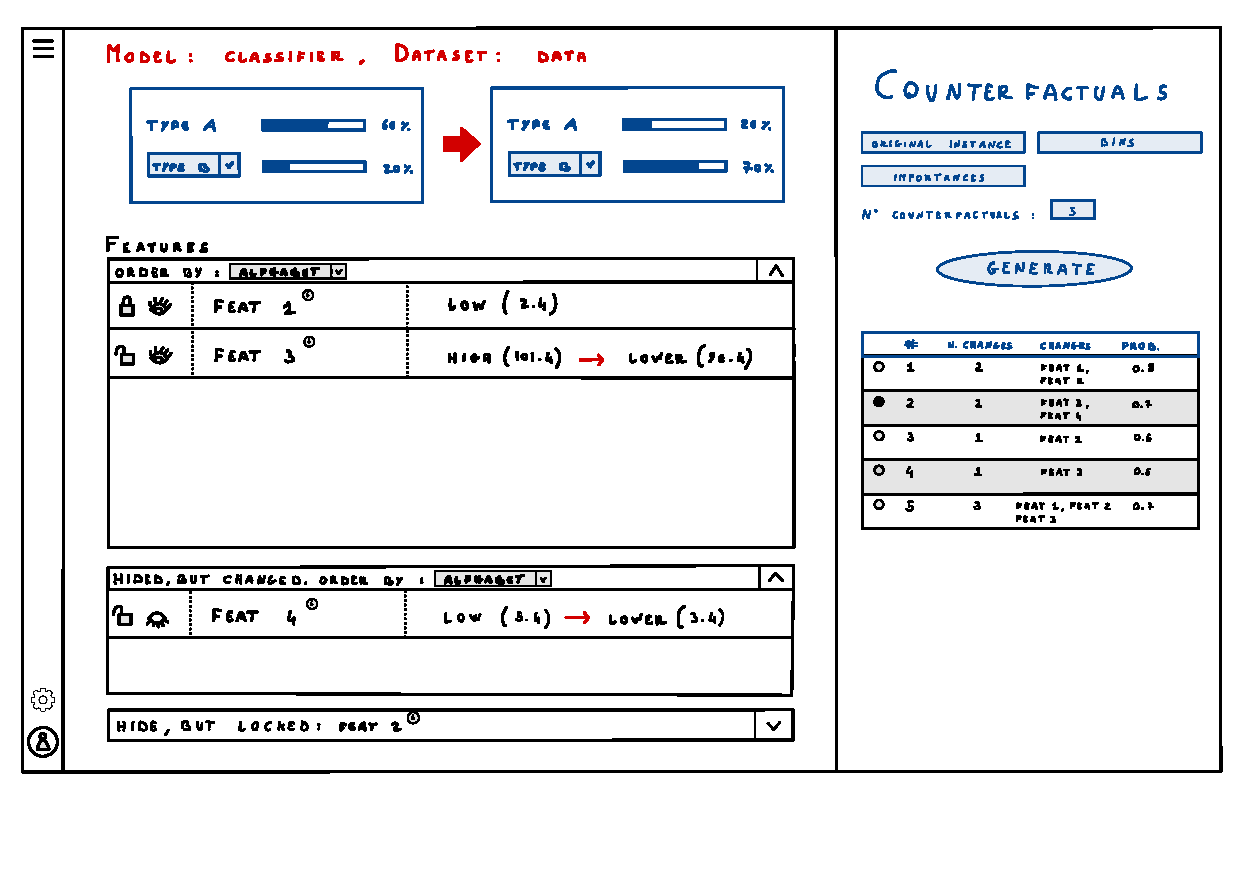
\includegraphics[width=\linewidth]{fig/counterfactual_main.pdf}
	\caption{Initial sketch of the final visualization.}
	\label{fig:main_page}
\end{figure}

\subsection*{Model-agnostic Counterfactual Generation}
A Django back-end is implemented to handle counterfactual generation requests. The back-end accepts \texttt{GET} requests containing an instance in JSON format and returns corresponding counterfactual examples. The system is model-agnostic, meaning that users can  upload their own trained models and datasets for generating counterfactual instances. The only requirement is that the model is differentiable. But, it can be argued that most non-differentiable models (Decision Trees, Rule based systems) are inherently more interpretable.

\subsection*{Model-Agnostic Binning}
To make the counterfactual explanations more interpretable, a model-agnostic binning method will be implemented. This transforms continuous feature values into discrete bins, aligning with the findings of Warren et al.~\cite{warren_et_al_user_study_2023} that show improved user understanding of counterfactual explanations with categorical features. We will use the local transformation method: CAT-CFLocal as described in~\cite{warren2022better}, where continuous feature values in the counterfactual instance are re-labelled as being "higher" or "lower" relative to the values in the original instance. 

%Todo: Compare different binnning techniques.

\subsection*{User Study}
While there exist many numerical evaluation metrics for counterfactual explanations, such as sparsity and proximity~\cite{keane2020good}, these measures are not suitable for evaluating the discretised counterfactual instances. Hence, a user study will be conducted to evaluate the effectiveness our proposed visualization method.

%Todo: Clearly define how the user study will be conducted.

